\chapter{Propuesta}\label{chapter:proposal}

Como propuesta de solución a la implementación de una API para los diferentes softwares de servidores DNS autoritarios de código abierto, se propone un arquitectura en la que API tiene acceso al sistema de almacenamiento de la configuración DNS para su manejo. Además existe un medio de comunicación entendible por la API y el servidor DNS para desarrollar cualquier intercambio de información necesario.

\begin{figure}[!ht]
    \centering
    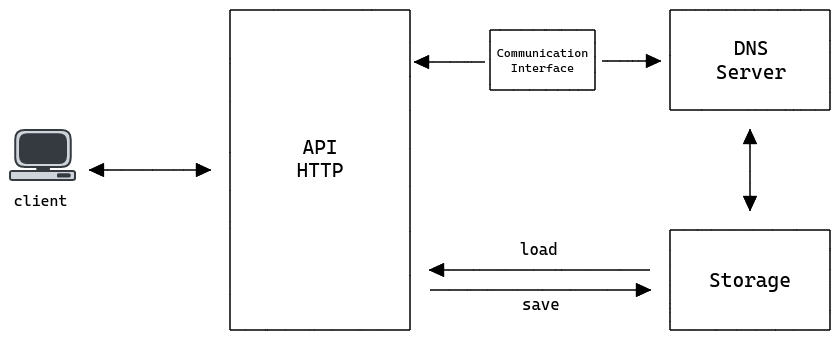
\includegraphics[width=\linewidth]{draws/proposal.png}
    \caption{Arquitectura de la propuesta.}
\end{figure}

La hipótesis teórica se basa en dos funciones: \verb+load+ para la lectura de los archivos de configuración desde un sistema de almacenamiento y \verb+save+ para la persistencia de los cambios realizados a dicho sistema. Estas funciones expuestas en una API HTTP, o similar, permiten realizar las funciones fundamentales de configuración sobre el servidor DNS.

En la sección 3.1 se describe el mecanismo carga de la configuración a través de la función \verb|load|. La sección 3.2 desarrolla el funcionamiento de \verb|save|, cómo esta asegura la correctitud de los cambios realizados en la configuración DNS y notifica al servidor DNS sobre estos.

\section{Lectura de la Configuración DNS}

Asumiendo que existe un servidor DNS autoritario $A$, con un sistema de persistencia en disco $S_A$. Sea $M_A$, la configuración del sistema DNS cargada por la API de $A$ y $r(S_A)$ una función capaz de leer y estructurar la información desde el sistema de almacenamiento $S_A$; se tiene la función \verb+load+ como se muestra a continuación.

\begin{algorithmic}
\Procedure{load}{$A$}
    \State $M_A \leftarrow r(S_A)$
\EndProcedure
\end{algorithmic}

\begin{figure}[!ht]
    \centering
    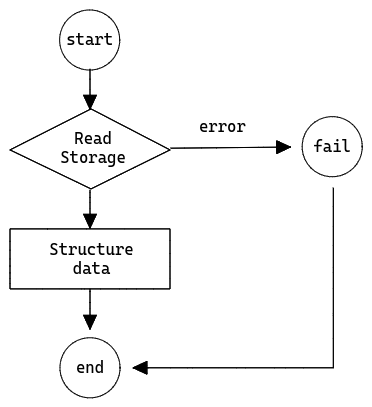
\includegraphics[width=0.5\linewidth]{draws/load.png}
    \caption{Diagrama de flujo para la función \textbf{load}.}
\end{figure}

\section{Escritura de la Configuración DNS}

Para definir \verb+save+, es necesario considerar que existe un bloqueo $L$ que limita el acceso de escritura (POST, PATCH, DELETE) a la API y $C_A$ un mecanismo de comunicación entre el servicio de la API y $A$. Sean $h(C_A)$ una función que indica a $A$ que su configuración en $S_A$ ha sido modificada, $f(M_A, u)$ la función que almacena de forma estructurada en el almacenamiento de la API las modificaciones $u$ enviados a esta y $g(S_A, u)$ la función que persiste el conjunto de modificaciones $u$ de forma estructurada en el sistema de almacenamiento de $A$. Entonces, se define \verb+save+ de la siguiente manera.

\begin{algorithmic}
\Procedure{save}{$A$, $u$}
    \State $M_A' \leftarrow f(M_A, u)$
    \State $g(S_A, u)$
    \State $h(C_A)$
    \State $M_A \leftarrow M_A'$
\EndProcedure
\end{algorithmic}

\begin{figure}[!ht]
    \centering
    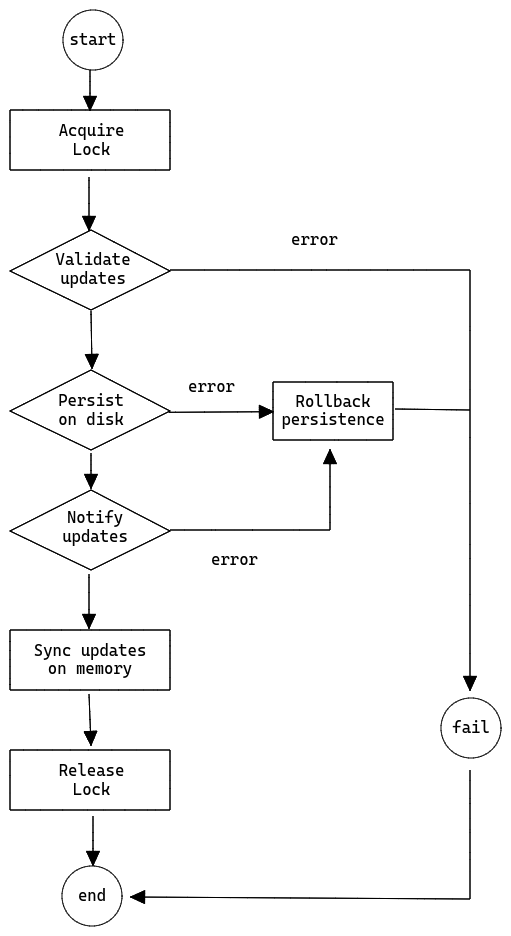
\includegraphics[width=0.6\linewidth]{draws/save.png}
    \caption{Diagrama de flujo para la función \textbf{save}.}
\end{figure}

Cuando se evalúa $f$ son realizadas las validaciones para garantizar que los cambios introducidos por $u$ son compatibles con el estado actual de $A$. En caso positivo, la actualización introducida por $u$ es persistida. Posteriormente, se notifica al servidor DNS que puede recargar su configuración. Si los estados posteriores (invocación a $g$ y $h$) a la validación de $u$ ocurren sin errores, se actualiza la información en $M_A$ para sincronizarla con los cambios realizados al servidor autoritario $A$.

